% !TEX root = ../thesis.tex

\chapter{Theory and Motivation for Searching for a Dibosonic Resonance}
\label{chap:theory}

\section{Introduction}

% History of QFT
Prior to the development of the Standard Model, attempts to reconcile quantum mechanics with special relativity resulted in the foundations for quantum field theory.
The first example of a successful quantum field theory is quantum electrodynamics (QED), which was principally developed by Richard Feynman and Julian Schwinger.
For their work in QED, they shared the 1965 Nobel Prize along with Sin-Itiro Tomonaga~\cite{NobelPrize:1965-Physics}.
To this day, it stands as one of the most precisely tested theories of physics, with quantities such as the anomalous magnetic dipole moment of the electron $a_e$ as predicted by QED agreeing with experiment by more than 10 significant digits~\cite{Aoyama_2015}.

% Development of the SM
However, while QED on its own is successful within its own domain of modeling electromagnetic interactions, it does not concern itself with the other two interactions of the Standard Model: the strong and weak nuclear forces.
The description of these two forces proved to be more mathematically complicated than QED, and the development of the quantum field theories that describe them did not come about until the 1960's and 1970's with the electroweak (EW) theory of Weinberg, Glashow, and Salam, and the theory of quantum chromodynamics (QCD) of Gell-Mann and Zweig.
EW theory and QCD also have their roots in Yang-Mills theory developed by Chen Ning Yang and Robert Mills in the 1950's~\cite{1954PhRv...96..191Y}, as they are both examples of non-abelian gauge theories.
The Standard Model is the resulting theory that came about by combining EW theory with QCD\footnotemark.
\footnotetext{While the theory itself began development in the 1960's, the term ``Standard Model'' was coined by Pais and Treiman in 1975~\cite{CaoFieldTheory}.}

% Problems with the SM
Today, the Standard Model remains as the dominant theory describing three of the four known forces, with gravity excluded due to its inability to be renormalized when approached as a quantum field theory.
The theory itself stands as one of the most well-tested models of physics in history, and all elementary particles predicted by the theory have been found, with the Higgs completing the family after being discovered in the summer of 2012. % Perhaps reword
However, despite the success of this theory, many fundamental questions of physics still remain unanswered.
As previously mentioned in chapter~\ref{chap:intro}, the theory does not include gravity, as it only accounts for the electromagnetic, strong, and weak nuclear forces.
It also does not account for the existence of Dark Matter or Dark Energy, and there are long-standing issues that the theory currently is incapable of addressing, such as the hierarchy problem~\cite{krippendorf2010cambridge}.
The theory is therefore regarded as incomplete, and efforts to find physics beyond the Standard Model are ongoing.

% Chapter overview
In this chapter, we briefly explore the main aspects of the Standard Model in section~\ref{sec:SM}, looking at the fundamental particles that it describes and some of its mathematical foundations.
Later, in section~\ref{sec:VBF}, we describe the theoretical background relevant to the search for a new fundamental particle beyond the Standard Model that this work presents.

\section{The Standard Model of Particle Physics}
\label{sec:SM}

% The standard model
The Standard Model is the prevailing theory in particle physics that classifies all known elementary particles, and describes how they interact with each other via the electromagnetic, weak, and strong forces.
Mathematically, the Standard Model is a gauge quantum field theory resulting from the combination of both EW theory and QCD.
Attempts at simply quantizing relativistic particles in the same way that nonrelativistic particles were quantized gives rise to problems such as negative-energy states and violations of causality~\cite{Peskin:257493}.
The need for the field description therefore arises from requiring that our theory obeys causality in the context of relativity, and that our theory allows for the creation and annihilation of particles.
Each elementary particle and antiparticle is associated with a field, individual particles are treated as excitations of the field, and the interactions between each of the different fields allow for the creation and annihilation of particles.

\subsection{The Elementary Particles}
\label{subsec:particles}

% The elementary particles
The Standard Model describes the interactions between 17 elementary particles, which are classified by quarks, leptons, gauge bosons, and scalar bosons.
A table of all particles described by the theory can be seen in figure~\ref{fig:standardModel}, labeled with their masses, charges, and spins~\cite{PhysRevD.98.030001}, with the fermions grouped by generation.
Quarks and leptons are classified as fermions since they have half-integer values for their spin, while the scalar and gauge bosons are eponymously named for the fact that they are bosons and therefore have integer values for their spin. % Check wording

\begin{figure}[htbp]
  \centering
  % !TEX root = ../../thesis.tex

\begin{tikzpicture}
  % Quarks
  \draw pic at (0,0) {particle={green!20}{$u$}{up}{$2.16$ MeV/$c^2$}{$2/3$}{$1/2$}};
  \draw pic at (0,-2.2) {particle={green!20}{$d$}{down}{$4.67$ MeV/$c^2$}{$-1/3$}{$1/2$}};
  \draw pic at (2.2,0) {particle={green!20}{$c$}{charm}{$1.27$ GeV/$c^2$}{$2/3$}{$1/2$}};
  \draw pic at (2.2,-2.2) {particle={green!20}{$s$}{strange}{$93$ MeV/$c^2$}{$-1/3$}{$1/2$}};
  \draw pic at (4.4,0) {particle={green!20}{$t$}{top}{$172.76$ GeV/$c^2$}{$2/3$}{$1/2$}};
  \draw pic at (4.4,-2.2) {particle={green!20}{$b$}{bottom}{$4.18$ MeV/$c^2$}{$-1/3$}{$1/2$}};

  % Leptons
  \draw pic at (0,-4.4) {particle={red!20}{$e$}{electron}{$511$ keV/$c^2$}{$-1$}{$1/2$}};
  \draw pic at (0,-6.6) {particle={red!20}{$\nu_e$}{$e$ neutrino}{$<1.1$ eV/$c^2$}{$0$}{$1/2$}};
  \draw pic at (2.2,-4.4) {particle={red!20}{$\mu$}{muon}{$105.66$ MeV/$c^2$}{$-1$}{$1/2$}};
  \draw pic at (2.2,-6.6) {particle={red!20}{$\nu_\mu$}{$\mu$ neutrino}{$<0.19$ eV/$c^2$}{$0$}{$1/2$}};
  \draw pic at (4.4,-4.4) {particle={red!20}{$\tau$}{tau}{$1.7769$ GeV/$c^2$}{$-1$}{$1/2$}};
  \draw pic at (4.4,-6.6) {particle={red!20}{$\nu_\tau$}{$\tau$ neutrino}{$<18.2$ MeV/$c^2$}{$0$}{$1/2$}};

  % Gauge Bosons
  \draw pic at (6.6,0) {particle={blue!20}{$g$}{gluon}{$0$}{$0$}{$1$}};
  \draw pic at (6.6,-2.2) {particle={blue!20}{$\gamma$}{photon}{$0$}{$0$}{$1$}};
  \draw pic at (6.6,-4.4) {particle={blue!20}{$Z$}{$Z$ boson}{$91.1876$ GeV/$c^2$}{$0$}{$1$}};
  \draw pic at (6.6,-6.6) {particle={blue!20}{$W$}{$W$ boson}{$80.379$ GeV/$c^2$}{$\pm1$}{$1$}};

  % Scalar Bosons
  \draw pic at (8.8,0) {particle={orange!20}{$H$}{higgs}{$124.97$ GeV/$c^2$}{0}{0}};

  % Labels
  \node at (-1,0.8) [anchor=mid east,scale=0.5] {mass};
  \node at (-1,0.5) [anchor=mid east,scale=0.5] {charge};
  \node at (-1,0.2) [anchor=mid east,scale=0.5] {spin};
  \coordinate (d) at (0,-2.2);
  \coordinate (nu) at (0,-6.6);
  \coordinate (w) at (6.6,-6.6);
  \coordinate (h) at (8.8,0);
  \coordinate (u) at (0,0);
  \coordinate (c) at (2.2,0);
  \coordinate (t) at (4.4,0);
  \node at ($(d)+(-1.35,-1)$) [rotate=90,anchor=mid west,text=green!100] {quarks};
  \node at ($(nu)+(-1.35,-1)$) [rotate=90,anchor=mid west,text=red!100] {leptons};
  \node at ($(w)+(1.35,-1)$) [rotate=90,anchor=mid west,text=blue!100] {gauge bosons};
  \node at ($(h)+(1.35,1)$) [rotate=90,anchor=mid east,text=orange!100] {scalar bosons};
  \node at ($(u)+(0,1.35)$) {I};
  \node at ($(c)+(0,1.35)$) {II};
  \node at ($(t)+(0,1.35)$) {III};
\end{tikzpicture}

  \caption{
    Table of all Standard Model particles grouped by generation and type, labeled with mass, charge, and spin.
    Particle types are colored green for quarks, red for leptons, blue for gauge bosons, and orange for scalar bosons.
  }
  \label{fig:standardModel}
\end{figure}

\subsubsection{Quarks}

% Quarks
Quarks are spin-1/2 particles that interact via the strong and weak nuclear forces, as well as the electromagnetic force.
The up and down quarks make up the protons and neutrons of everyday matter that we see and interact with.
For example, a proton is made up of two $u$'s and one $d$ ($uud$), while a neutron is made of two $d$'s and one $u$ ($ddu$).
These are just two of the many different combinations of composite particles that can be formed by quarks.

% Combinations of quarks
There are two main combinations of quarks to consider: mesons and baryons.
Mesons are composed of one quark and an antiquark, and baryons are composed of three quarks or three antiquarks. % Mention recently observed pentaquark?
For example, pions ($\pi^0$/$\pi^\pm$) were the first mesons to be observed, and can be electrically charged when comprised only of up or down quark-antiquark pairs (i.e., a $\pi^+$ is made from the combination $u\bar{d}$, and a $\pi^-$ is made from $d\bar{u}$), or it can be electrically neutral (i.e., a $\pi^0$ is made from $u\bar{u}$ or $d\bar{d}$).
On the other hand, protons and neutrons are examples of baryons, as they are each made of three quarks.
Both baryons and mesons are examples of hadrons: bound states of quarks.

% Color charge
One unique aspect of quarks is that they carry color charge, and all hadrons are considered `colorless' states.
The three quarks in a baryon have red, green, and blue (or antired, antigreen, and antiblue) charge to form a colorless combination, and mesons can come in pairs of red and antired, green and antigreen, and blue and antiblue.
This phenomenon is known as color confinement, and while there is currently no analytic proof of color confinement in QCD, no colorless configuration of quarks has been observed~\cite{muta2010foundations}.

\subsubsection{Leptons}

% leptons
Leptons, like quarks, are also spin-1/2 particles that can be electrically charged. Unlike quarks, they only interact via the electromagnetic and weak nuclear forces.
The electron is the most familiar lepton, as it is a component of the atoms that are found in everyday interactions.
However, it also has two heavier cousins: the muon and the tau.
Both of these particles have the same charge as the electron, but their masses are much larger.
Finally, leptons also include neutrinos, which are extremely light particles that have no electric charge, and therefore only interact via the weak force.
% Possibly elaborate

\subsubsection{Gauge Bosons}

% Gauge bosons
The gauge bosons include the gluon, the photon, and the $W$ and $Z$ bosons.
Each gauge boson is a spin-1 particle that mediates the three fundamental interactions that the Standard Model describes.
Gluons are massless particles that mediate the strong nuclear force, and they only interact with quarks since they are the only particles to carry color charge.
Photons are the most familiar example of the gauge bosons, as we can quite literally see them since light is made of photons.
They are masses particles that mediate the electromagnetic force, and they interact with any particle that is electrically charged.
Finally, the $Z$ and $W$ bosons are massive particles that mediate the weak nuclear force, which is responsible for radioactive decay.
% Possibly elaborate

\subsubsection{Scalar Bosons}

% Scalar bosons
The last category of bosons to consider is the scalar bosons, which are spin-0 particles.
This family contains only one member: the Higgs boson.
The need for the Higgs boson arises due to the fact that all of the previously mentioned particles do not have intrinsic masses.
Rather, the Higgs is responsible for giving all massive Standard Model particles their masses, with the exception of the neutrinos.
This occurs through the Higgs mechanism, in which spontaneous symmetry breaking and gauge invariance cause the Higgs field to interact with the other fields in the Standard model, thereby imparting the observed masses onto the particles. % Check wording

\subsection{Mathematical Structure of the Standard Model}

% The mathematical structure of the standard model
As the Standard Model is a quantum field theory, it has a Lagrangian density $\mathcal{L}_\mathrm{SM}$ that contains all the information about the fields corresponding to each particle and how they interact with each other.
Each term in this Lagrangian must be Lorentz invariant in order for the Lagrangian to remain the same under gauge transformations or boosts and rotations.
The terms present in $\mathcal{L}_\mathrm{SM}$ allow us to compute probability amplitudes for particle production and decay processes through the method of Feynman diagrams.
The Standard Model is also a non-abelian gauge theory, in which the internal symmetry group is $SU(3)_C\times SU(2)_L\times U(1)_Y$~\cite{Srednicki:1019751}.
The $SU(3)_C$ symmetry group corresponds to the QCD interactions of the quarks and gluons, while the $SU(2)_L\times U(1)_Y$ group corresponds to the electroweak interactions.
The symmetries of these groups lead to conservation of color charge $C$, weak isospin $T_3$, and weak hypercharge $Y_W$. %\footnotemark. % Check wording
%\footnotetext{Electric charge $Q$ arises as a linear combination of $T_3$ and $Y_W$ given by $Q=T_3+\frac{1}{2}Y_W$.}

\subsubsection{Lagrangian Formalism}

% The QED Lagrangian
A simple yet illustrative example of a Lagrangian for a quantum field theory is that of QED for a spin-1/2 field~\cite{Klauber:2013ipa}:
\begin{equation}\label{eq:QED}
  \mathcal{L}_\mathrm{QED}=-\frac{1}{4}F_{\mu\nu}F^{\mu\nu}+\bar{\psi}(i\gamma^\mu D_\mu-m)\psi.
\end{equation}
Here, $\psi$ is a spin-1/2 field, $\bar{\psi}\equiv\psi^\dagger\gamma^0$ is the Dirac adjoint for $\psi$, $F^{\mu\nu}=\partial^\mu A^\nu-\partial^\nu A^\mu$ is the electromagnetic field strength tensor, $D_\mu=\partial_\mu+ieA_\mu$ is the gauge covariant derivative, $\gamma^\mu$ is the set of Dirac matrices, and $m$ is the mass of the particle corresponding to the field $\psi$.

% Equations of motion
The classical equations of motion for the fields can be obtained through the Euler-Lagrange equation for a field $\phi$, which is given by
\begin{equation}\label{eq:EL}
  \pdv{\mathcal{L}}{\phi}-\partial_\mu\pqty{\pdv{\mathcal{L}}{(\partial_\mu\phi)}}=0.
\end{equation}
Applying equation~\ref{eq:EL} to the spin-1/2 field $\psi$ yields
\begin{equation}
  i\gamma^\mu D_\mu\psi-m\psi=0
\end{equation}
which is the Dirac equation with the gauge covariant derivative in place of the usual partial derivative.
On the other hand, for $A^\mu$, we get
\begin{equation}
  \partial_\mu F^{\mu\nu}=e\bar{\psi}\gamma^\mu\psi,
\end{equation}
which are the inhomogeneous Maxwell equations for the electromagnetic field.

\subsubsection{Feynman Diagrams}

% Feynman diagrams
Feynman diagrams are pictorial representations of the terms in present in the Dyson series, which is a perturbative expansion of the time evolution operator in the interaction picture.
Through the process of canonical quantization, one may obtain a quantum field theory starting from a Lagrangian $\mathcal{L}$~\cite{Lancaster:1629337}.
The Lagrangian contains all the information about how the fields interact with one another, and from this we may obtain the Feynman rules to compute scattering amplitudes and cross-sections.

% Example with QED Lagrangian
For example, given the QED Lagrangian $\mathcal{L}_\mathrm{QED}$ in equation~\ref{eq:QED}, we obtain the following Feynman rules~\cite{Schwartz:2013pla}:
\begin{equation}
  \begin{aligned}
    % !TEX root = ../../thesis.tex
\begin{tikzpicture}[baseline=\eqheight]
  \begin{feynman}
    % Lines
    \draw[boson] (-0.75,0) -- (0.75,0);
    \draw[->] (-0.5,0.25) -- (0.5,0.25) node[above,pos=0.5] {$p$};
  \end{feynman}
\end{tikzpicture}
 &= \frac{-ig_{\mu\nu}}{p^2+i\epsilon}, & % !TEX root = ../../thesis.tex
\begin{tikzpicture}[baseline=\eqheight]
  \begin{feynman}
    % Lines
    \draw[boson] (-0.75,0) -- (0.75,0);
    \draw[->] (-0.5,0.25) -- (0.5,0.25) node[above,pos=0.5] {$p$};
    \fill[white] (0.75,0) circle (0.2);
    \draw[pattern=north west lines] (0.75,0) circle (0.2);
  \end{feynman}
\end{tikzpicture}
 &= \epsilon_\mu(p), & % !TEX root = ../../thesis.tex
\begin{tikzpicture}[baseline=\eqheight]
  \begin{feynman}
    % Lines
    \draw[boson] (-0.75,0) -- (0.75,0);
    \draw[->] (-0.5,0.25) -- (0.5,0.25) node[above,pos=0.5] {$p$};
    \fill[white] (-0.75,0) circle (0.2);
    \draw[pattern=north west lines] (-0.75,0) circle (0.2);
  \end{feynman}
\end{tikzpicture}
 &= \epsilon_\mu^*(p),\\
    % !TEX root = ../../thesis.tex
\begin{tikzpicture}[baseline=\eqheight]
  \begin{feynman}
    % Lines
    \draw[fermion] (0.75,0) -- (-0.75,0);
    \draw[->] (-0.5,0.25) -- (0.5,0.25) node[above,pos=0.5] {$p$};
  \end{feynman}
\end{tikzpicture}
 &= \frac{i(\slashed{p}+m)}{p^2-m^2+i\epsilon}, & % !TEX root = ../../thesis.tex
\begin{tikzpicture}[baseline=\eqheight]
  \begin{feynman}
    % Lines
    \draw[fermion] (-0.75,0) -- (0.75,0);
    \draw[->] (-0.5,0.25) -- (0.5,0.25) node[above,pos=0.5] {$p$};
    \fill[white] (0.75,0) circle (0.2);
    \draw[pattern=north west lines] (0.75,0) circle (0.2);
  \end{feynman}
\end{tikzpicture}
 &= u^s(p), & % !TEX root = ../../thesis.tex
\begin{tikzpicture}[baseline=\eqheight]
  \begin{feynman}
    % Lines
    \draw[fermion] (-0.75,0) -- (0.75,0);
    \draw[->] (-0.5,0.25) -- (0.5,0.25) node[above,pos=0.5] {$p$};
    \fill[white] (-0.75,0) circle (0.2);
    \draw[pattern=north west lines] (-0.75,0) circle (0.2);
  \end{feynman}
\end{tikzpicture}
 &= \bar{u}^s(p),\\
    % !TEX root = ../../thesis.tex
\begin{tikzpicture}[baseline=\eqheight]
  \begin{feynman}
    % Lines
    \draw[boson] (0,0) -- (90:0.866);
    \draw[fermion] (0,0) -- (210:0.866);
    \draw[anti fermion] (0,0) -- (330:0.866);
  \end{feynman}
\end{tikzpicture}
 &= -ie\gamma^\mu, & % !TEX root = ../../thesis.tex
\begin{tikzpicture}[baseline=\eqheight]
  \begin{feynman}
    % Lines
    \draw[fermion] (0.75,0) -- (-0.75,0);
    \draw[->] (-0.5,0.25) -- (0.5,0.25) node[above,pos=0.5] {$p$};
    \fill[white] (0.75,0) circle (0.2);
    \draw[pattern=north west lines] (0.75,0) circle (0.2);
  \end{feynman}
\end{tikzpicture}
 &= \bar{v}^s(p), & % !TEX root = ../../thesis.tex
\begin{tikzpicture}[baseline=\eqheight]
  \begin{feynman}
    % Lines
    \draw[fermion] (0.75,0) -- (-0.75,0);
    \draw[->] (-0.5,0.25) -- (0.5,0.25) node[above,pos=0.5] {$p$};
    \fill[white] (-0.75,0) circle (0.2);
    \draw[pattern=north west lines] (-0.75,0) circle (0.2);
  \end{feynman}
\end{tikzpicture}
 &= v^s(p).
  \end{aligned}
\end{equation}
These rules may then immediately be applied to a process such as $e^-e^+\to\mu^-\mu^+$ to obtain the first-order scattering amplitude,
\begin{equation}
  i\mathcal{M}=% !TEX root = ../../thesis.tex
\begin{tikzpicture}[baseline=\eqheight]
  \begin{feynman}
    % Vertices
    \coordinate (f1) at (135:1.5);
    \coordinate (f2) at (225:1.5);
    \coordinate (b1) at (0,0);
    \coordinate (b2) at (1.5,0);
    \coordinate (f3) at ($(b2)+(45:1.5)$);
    \coordinate (f4) at ($(b2)+(-45:1.5)$);

    % Lines
    \draw[fermion] (f1) -- (b1);
    \draw[fermion] (b1) -- (f2);
    \draw[boson] (b1) -- (b2) node[pos=0.5,above] {$\gamma$};
    \draw[fermion] (b2) -- (f3);
    \draw[fermion] (f4) -- (b2);
    \draw[->] ($(135:1.25)+(45:0.25)$) -- ($(135:0.25)+(45:0.25)$) node[pos=0.5,above right] {$p_1$};
    \draw[->] ($(225:1.25)+(-45:0.25)$) -- ($(225:0.25)+(-45:0.25)$) node[pos=0.5,below right] {$p_2$};
    \draw[->] ($(b2)+(45:0.25)+(135:0.25)$) -- ($(b2)+(45:1.25)+(135:0.25)$) node[pos=0.5,above left] {$p_3$};
    \draw[->] ($(b2)+(-45:0.25)+(225:0.25)$) -- ($(b2)+(-45:1.25)+(225:0.25)$) node[pos=0.5,below left] {$p_4$};

    % Labels
    \node[anchor=mid,left] at (f1) {$e^-$};
    \node[anchor=mid,left] at (f2) {$e^+$};
    \node[anchor=mid,right] at (f3) {$\mu^-$};
    \node[anchor=mid,right] at (f4) {$\mu^+$};
  \end{feynman}
\end{tikzpicture}
=\frac{ie^2}{(p_1+p_2)^2}\bqty{\bar{v}(p_2)\gamma^\mu u(p_1)}\bqty{\bar{u}(p_3)\gamma_\mu v(p_4)}.
\end{equation}
This can then be used to compute the scattering cross-section. For a process in the center-of-mass frame with two particles in the initial state with momenta $\mathbf{p}_1=-\mathbf{p_2}$, and two particles in the final state with momenta $\mathbf{p}_3=-\mathbf{p}_4$.
The cross-section assuming unpolarized scattering is
\begin{align*}
  \dv{\sigma(e^-e^+\to\mu^-\mu^+)}{\Omega} &= \frac{1}{64\pi^2E^2_\mathrm{CM}}\frac{|\mathbf{p}_f|}{|\mathbf{p}_i|}\sum_\mathrm{spins}|\mathcal{M}|^2\\
  &= \frac{\alpha^2}{4E_\mathrm{CM}^2}\sqrt{1-\frac{m_\mu^2}{E^2}}\bqty{1+\frac{m_\mu^2}{E^2}+\pqty{1-\frac{m_\mu^2}{E^2}}\cos^2\theta},
  \numberthis
\end{align*}
where $|\mathbf{p}_i|\equiv|\mathbf{p}_1|=|\mathbf{p}_2|$ and $|\mathbf{p}_f|\equiv|\mathbf{p}_3|=|\mathbf{p}_4|$, $E_\mathrm{CM}$ is the total energy in the center-of-mass frame, $E=E_\mathrm{CM}/2$ is the energy of one of the incoming or outgoing particles, $\theta$ is measured with respect to the axis of the initial momenta, and $m_\mu$ is the mass of the muon.

% Feynman diagrams generalized to the standard model
The process for obtaining scattering cross-sections for other field theories with a specified Lagrangian $\mathcal{L}$ is similar.
Thus, applying this machinery to the SM Lagrangian allows us to construct the diagrams necessary to compute scattering amplitudes and cross-sections for any particular process of interest. Some examples of SM vertices may be seen in figure~\ref{fig:SMVert}~\cite{Romao_2012}.

\begin{figure}[htbp]
  \centering
  % !TEX root = ../../thesis.tex
\begin{tikzpicture}
  \begin{feynman}
    % gluon-quark vertex
    \coordinate (d1) at (-3.5,3.5);
    \draw[gluon] (d1) -- ($(d1)+(90:1.601)$) node[pos=0.9,right] {$g$};
    \draw[anti fermion] (d1) -- ($(d1)+(210:1.299)$) node[pos=0.9,below left] {$q$};
    \draw[fermion] (d1) -- ($(d1)+(330:1.299)$) node[pos=0.9,below right] {$q$};

    % 3-gluon vertex
    \coordinate (d2) at (0,3.5);
    \draw[gluon] (d2) -- ($(d2)+(90:1.601)$) node[pos=0.9,right] {$g$};
    \draw[gluon] (d2) -- ($(d2)+(210:1.299)$) node[pos=0.9,below left] {$g$};
    \draw[gluon] (d2) -- ($(d2)+(330:1.299)$) node[pos=0.9,below right] {$g$};

    % 4-gluon vertex
    \coordinate (d3) at (3.5,3.5+0.475);
    \draw[gluon] (d3) -- ($(d3)+(-1.125,1.125)$) node[pos=0.9,below left] {$g$};
    \draw[gluon] (d3) -- ($(d3)+(1.125,1.125)$) node[pos=0.9,above left] {$g$};
    \draw[gluon] (d3) -- ($(d3)+(-1.125,-1.125)$) node[pos=0.9,below right] {$g$};
    \draw[gluon] (d3) -- ($(d3)+(1.125,-1.125)$) node[pos=0.9,above right] {$g$};

    % photon-charge vertex
    \coordinate (d4) at (-3.5,0);
    \draw[boson] (d4) -- ($(d4)+(90:1.601)$) node[pos=0.9,right] {$\gamma$};
    \draw[anti fermion] (d4) -- ($(d4)+(210:1.299)$) node[pos=0.9,below left] {$f_Q$};
    \draw[fermion] (d4) -- ($(d4)+(330:1.299)$) node[pos=0.9,below right] {$f_Q$};

    % W-lepton vertex
    \coordinate (d5) at (0,0);
    \draw[boson] (d5) -- ($(d5)+(90:1.601)$) node[pos=0.9,right] {$W$};
    \draw[anti fermion] (d5) -- ($(d5)+(210:1.299)$) node[pos=0.9,below left] {$\ell$};
    \draw[fermion] (d5) -- ($(d5)+(330:1.299)$) node[pos=0.9,below right] {$\nu_\ell$};

    % 4-W/Z vertex
    \coordinate (d6) at (3.5,0.475);
    \draw[boson] (d6) -- ($(d6)+(-1.125,1.125)$) node[pos=0.9,below left] {$W$};
    \draw[boson] (d6) -- ($(d6)+(1.125,1.125)$) node[pos=0.9,above left] {$W$};
    \draw[boson] (d6) -- ($(d6)+(-1.125,-1.125)$) node[pos=0.9,below right] {$W/Z/\gamma$};
    \draw[boson] (d6) -- ($(d6)+(1.125,-1.125)$) node[pos=0.9,above right] {$W/Z/\gamma$};

    % Z-fermion vertex
    \coordinate (d7) at (-3.5,-3.5);
    \draw[boson] (d7) -- ($(d7)+(90:1.601)$) node[pos=0.9,right] {$Z$};
    \draw[anti fermion] (d7) -- ($(d7)+(210:1.299)$) node[pos=0.9,below left] {$f$};
    \draw[fermion] (d7) -- ($(d7)+(330:1.299)$) node[pos=0.9,below right] {$f$};

    % W-quark vertex
    \coordinate (d8) at (0,-3.5);
    \draw[boson] (d8) -- ($(d8)+(90:1.601)$) node[pos=0.9,right] {$W$};
    \draw[anti fermion] (d8) -- ($(d8)+(210:1.299)$) node[pos=0.9,below left] {$q_u$};
    \draw[fermion] (d8) -- ($(d8)+(330:1.299)$) node[pos=0.9,below right] {$q_d$};

    % W-Z/photon vertex
    \coordinate (d9) at (3.5,-3.5);
    \draw[boson] (d9) -- ($(d9)+(90:1.601)$) node[pos=0.9,right] {$Z/\gamma$};
    \draw[boson] (d9) -- ($(d9)+(210:1.299)$) node[pos=0.9,below left] {$W$};
    \draw[boson] (d9) -- ($(d9)+(330:1.299)$) node[pos=0.9,below right] {$W$};
  \end{feynman}
\end{tikzpicture}

  \caption{
    Examples of vertices for constructing Feynman diagrams in the Standard Model, where $f$ is any fermion, $f_Q$ is any electrically charged fermion, $\ell$ is any lepton that is not a neutrino, $q_u$ is an up-type quark ($u$, $c$, $t$), and $q_d$ is a down-type quark ($d$, $s$, $b$).
    For the quartic electroweak vertex, the two particles interacting with the $W$'s must be chosen such that charge conservation holds.
  }
  \label{fig:SMVert}
\end{figure}

\subsubsection{Gauge Theory}

% Gauge theory
One of the most foundational aspects of the Standard Model is the notion of gauge invariance, which means that the Lagrangian $\mathcal{L}$ remains invariant under a set of transformations.
The invariance of the Lagrangian under these transformations leads to conservation laws as a consequence of Noether's theorem.
This is at the heart of the Standard Model and why it is a $SU(3)_C\times SU(2)_L\times U(1)_Y$ gauge theory.

% Example with Dirac Lagrangian
To see this, consider the Dirac Lagrangian for a spin-1/2 field given by
\begin{equation}
  \mathcal{L}_\mathrm{Dirac}=\bar{\psi}(i\gamma^\mu\partial_\mu-m)\psi.
\end{equation}
This Lagrangian is invariant under the global $U(1)$ transformation $\psi\to e^{i\alpha}\psi$, as $\bar{\psi}\to e^{-i\alpha}\bar{\psi}$ and the product $\bar{\psi}\psi$ remains the same.
However, if we insist on a local $U(1)$ transformation such that $\psi\to e^{i\alpha(x)}\psi$, then the invariance is broken since we now have
\begin{equation}
  \bar{\psi}\gamma^\mu\partial_\mu\psi\to e^{-i\alpha(x)}\bar{\psi}\gamma^\mu\partial_\mu\bqty{e^{i\alpha(x)}\psi}=\bar{\psi}\gamma^\mu\partial_\mu\psi+\bar{\psi}\gamma^\mu[i\partial_\mu\alpha(x)]\psi,
\end{equation}
and hence
\begin{equation}
  \mathcal{L}\to\mathcal{L}-\bar{\psi}\gamma^\mu[\partial_\mu\alpha(x)]\psi.
\end{equation}

% Introducing the gauge field
However, the symmetry can be restored by adding an interaction term with a gauge field $A_\mu$ in the Lagrangian and demanding that it transform along with $\psi$ according to
\begin{equation}
  A_\mu\to A_\mu-\frac{1}{e}\partial_\mu\alpha(x),
\end{equation}
with an interaction Lagrangian
\begin{equation}
  \mathcal{L}_\mathrm{int}=-e\bar{\psi}\gamma^\mu A_\mu\psi.
\end{equation}
But introducing the gauge field requires that we also add a kinetic term for $A_\mu$ of the form
\begin{equation}
  \mathcal{L}_\mathrm{kin}=-\frac{1}{4}F_{\mu\nu}F^{\mu\nu},
\end{equation}
with $F^{\mu\nu}=\partial^\mu A^\nu-\partial^\nu A^\mu$.
Then the full Lagrangian is now
\begin{equation}
  \mathcal{L}=-\frac{1}{4}F_{\mu\nu}F^{\mu\nu}+\bar{\psi}(i\gamma^\mu\partial_\mu-m)\psi-e\bar{\psi}\gamma^\mu A_\mu\psi=-\frac{1}{4}F_{\mu\nu}F^{\mu\nu}+\bar{\psi}(i\gamma^\mu D_\mu-m)\psi,
\end{equation}
where $D_\mu=\partial_\mu+ieA_\mu$ is the usual gauge covariant derivative.
This is in fact the QED Lagrangian of equation~\ref{eq:QED}.
Thus, $\mathcal{L}_\mathrm{QED}$ is exhibits a local $U(1)$ symmetry, and applying Noether's theorem to the $U(1)$ gauge transformations reveals that the conserved quantity under this symmetry is electric charge.

% Gauge theory applied to the standard model
This same process can be applied to the overall $SU(3)_C\times SU(2)_L\times U(1)_Y$ gauge group to obtain conservation of color charge $C$, weak isospin $T_3$, and weak hypercharge $Y_W$.
The method of introducing a gauge field and replacing ordinary derivatives with gauge covariant derivatives to obtain local gauge symmetry is known as the minimal coupling rule~\cite{cheng1984}.
While the example of local $U(1)$ symmetry with the QED Lagrangian is simpler due to the fact that $U(1)$ is an abelian group, the process is similar for the non-abelian groups such as $SU(3)$ and $SU(2)$.
The number of generators for the gauge group corresponds to the number of gauge fields that are introduced to the Lagrangian.
For example, the EW symmetry group $SU(2)_L\times U(1)_Y$ has four generators, each of which correspond to the four EW bosons ($W^+$, $W^-$, $Z$, $\gamma$).
Thus, the gauge bosons are named for the fact that their fields naturally arise from demanding local gauge symmetry for our Lagrangian.

\subsubsection{The Higgs Mechanism}

% The need for the Higgs mechanism
One lingering issue arising from introducing the gauge fields is that the fields are required to be massless, otherwise the mass terms arising from the fields would spoil the gauge invariance.
For QCD this is not an issue since gluons are massless.
However, for EW theory this is a problem since the photon is massless, but the $W^\pm$ and $Z$ bosons are not.

% Example with a simple model
The Higgs mechanism solves this through spontaneous symmetry breaking by introducing a scalar field that interacts with the gauge fields in such a way that the masses are imparted onto them.
To see this mechanism in action, we may consider a simple model with a complex scalar field $\phi=\phi_1+i\phi_2$ with the following Lagrangian~\cite{GriffithsParticle}:
\begin{equation}
  \mathcal{L}=\frac{1}{2}(\partial_\mu\phi)^*(\partial^\mu\phi)+\frac{1}{2}\mu^2(\phi^*\phi)-\frac{1}{4}\lambda^2(\phi^*\phi)^2.
\end{equation}
By inspection, this Lagrangian has a $U(1)$ global symmetry under the transformation $\phi\to e^{i\theta}\phi$.
However, in order to apply perturbation theory so that we may use Feynman diagrams to compute scattering amplitudes, the Lagrangian must be defined so that the fields are shifted to the global minimum of the potential\footnotemark.
\footnotetext{The potential in this case is $\mathcal{U}(\phi,\phi^*)=-\frac{1}{2}\mu^2(\phi^*\phi)+\frac{1}{4}\lambda^2(\phi^*\phi)^2$ since $\mathcal{L}=\mathcal{T}-\mathcal{U}$.}
We may do so by noticing that the minimum of the potential lies on a circle of radius $\mu/\lambda$ in $(\phi_1,\phi_2)$ space, and rewriting $\mathcal{L}$ in terms of new fields $\eta$ and $\xi$ defined by
\begin{equation}\label{eq:fields}
  \eta=\phi_1-\mu/\lambda,\qquad \xi=\phi_2,
\end{equation}
and the Lagrangian is now
\begin{equation}
  \begin{aligned}
    \mathcal{L} &= \frac{1}{2}(\partial_\mu\xi)(\partial^\mu\xi)+\frac{1}{2}(\partial_\mu\eta)(\partial^\mu\eta)-\mu^2\eta^2\\
    &\equad- \bqty{\mu\lambda(\eta^3+\eta\xi^2)+\frac{\lambda^2}{4}(\eta^4+\xi^4+2\eta^2\xi^2)}+\frac{\mu^2}{4\lambda^2}.
  \end{aligned}
\end{equation}
Reading off the quadradic terms in $\mathcal{L}$ reveals that the fields have acquired masses $m_\eta=\sqrt{2}\mu$ and $m_\xi=0$.

% Spontaneous symmetry breaking
However, the Lagrangian no longer exhibits the global $U(1)$ symmetry that was present when written in terms of $\phi$ and $\phi^*$, and there is now a massless field $\xi$ present.
This phenomenon in which the original symmetry is no longer present is known as spontaneous symmetry breaking, and the introduction of a massless scalar field is a consequence of Goldstone's theorem, which states that the spontaneous breaking of a continuous global symmetry is accompanied by the presence of a massless Goldstone boson~\cite{PhysRev.127.965}.
Evidently, $\xi$ is the Goldstone boson present in the theory.

% Local gauge symmetry revisted
We may repeat this process but instead promote the original global $U(1)$ symmetry to a local symmetry and take the usual approach of introducing a gauge field $A^\mu$ and gauge covariant derivative $D_\mu=\partial_\mu+ieA_\mu$.
Our Lagrangian is now
\begin{equation}
  \mathcal{L}=-\frac{1}{4}F_{\mu\nu}F^{\mu\nu}+\frac{1}{2}(D_\mu\phi)^*(D^\mu\phi)+\frac{1}{2}\mu^2(\phi^*\phi)-\frac{1}{4}\lambda^2(\phi^*\phi)^2.
\end{equation}
and if we apply the same shift in the fields in equation~\ref{eq:fields} so that the potential is instead written about the minimum, we obtain
\begin{equation}
  \begin{aligned}
    \mathcal{L} &= \frac{1}{2}(\partial_\mu\xi)(\partial^\mu\xi)+\frac{1}{2}(\partial_\mu\eta)(\partial^\mu\eta)-\mu^2\eta^2-\frac{1}{4}F_{\mu\nu}F^{\mu\nu}+\frac{1}{2}\frac{e^2\mu^2}{\lambda^2}A_\mu A^\mu\\
    &\equad+ e[\eta(\partial_\mu\xi)-\xi(\partial_\mu\eta)]A^\mu+\frac{e^2\mu}{\lambda}\eta A_\mu A^\mu+\frac{1}{2}e^2(\xi^2+\eta^2)A_\mu A^\mu\\
    &\equad- \lambda\mu(\eta^3+\eta\xi^2)-\frac{1}{4}\lambda^2(\eta^4+2\eta^2\xi^2+\xi^4)+\frac{e\mu}{\lambda}(\partial_\mu\xi)A^\mu+\frac{\mu^4}{4\lambda^2}.
  \end{aligned}
\end{equation}
Again we have a massive $\eta$ field, and now the gauge field $A^\mu$ has acquired a mass $m_A=e\mu/\lambda$.
But there are two problems: the Goldstone boson $\xi$ is still present, and there is now a term in $\mathcal{L}$ of the form $(\partial_\mu\xi)A^\mu$.
Any term in the Lagrangian that is bilinear in two different fields indicates that $\mathcal{L}$ is not written in terms of fields corresponding to physical particles.

% The Higgs mechanism in action
Both issues are resolved by applying a gauge transformation to the original fields $\phi$ and $\phi^*$ so that $\phi\to e^{i\theta}\phi$ and $\phi^*\to e^{-i\theta}\phi^*$, with $\theta=-\arctan(\phi_2/\phi_1)$.
This is equivalent to setting $\phi_2=0$, which means that $\xi=0$ as well.
Since the Lagrangian is invariant under the $U(1)$ gauge transformation, we are left with all terms that do not contain $\xi$, and hence
\begin{equation}
  \begin{aligned}
    \mathcal{L} &= \frac{1}{2}(\partial_\mu\eta)(\partial^\mu\eta)-\mu^2\eta^2-\frac{1}{4}F_{\mu\nu}F^{\mu\nu}+\frac{1}{2}\frac{e^2\mu^2}{\lambda^2}A_\mu A^\mu+\frac{e^2\mu}{\lambda}\eta A_\mu A^\mu\\
    &\equad+ \frac{1}{2}e^2\eta^2A_\mu A^\mu-\lambda\mu\eta^3-\frac{1}{4}\lambda^2\eta^4+\frac{\mu^4}{4\lambda^2}.
  \end{aligned}
\end{equation}
Thus, the Goldstone boson is eliminated, we are left with the massive scalar field $\eta$ and the massive gauge field $A^\mu$, and the gauge field has also acquired a longitudinal polarization state in the process.

% The Higgs mechanism applied to the standard model
The Higgs mechanism is ultimately the result of combining spontaneous symmetry breaking and local gauge invariance~\cite{Higgs:1964ia}, and applying this process to the $SU(2)_L\times U(1)_Y$ EW theory accounts for the masses of the electroweak $W^\pm$ and $Z$ bosons, while also introducing the Higgs field itself.
It is for this reason that discovering the Higgs was of the utmost importance in verifying the Standard Model's description of the electroweak sector.
Meanwhile, the fermions gain their masses through a Yukawa interaction with the Higgs field.

\subsection{Beyond the Standard Model}
\label{subsec:BSM}

% Overview of BSM
The incompleteness of the Standard Model has driven theoretical developments of alternative models that resolve its shortcomings~\cite{2010arXiv1005.1676L}.
A few examples are Grand Unified Theories, supersymmetry (SUSY), and models based on extra spatial dimensions.
While such theories are currently of high interest due to the prospect of superseding the Standard Model, some are based on developments that predate the Standard Model itself.

\subsubsection{The Hierarchy Problem}

% The hierarchy problem
One major outstanding issue of interest relevant to this work is the inability of the Standard Model to deal with the hierarchy problem.
Using three fundamental constants, one may define the Planck mass as
\begin{equation}
  m_P=\sqrt{\frac{\hbar c}{G}}\approx1.22\times10^{19}\unit{MeV/\clight^2},
\end{equation}
where $\hbar$ is the reduced Planck constant, $c$ is the speed of light, and $G$ is Newton's gravitational constant.
This defines an energy scale at which effects due to gravity would become apparent in particle physics experiments~\cite{QFTNutshell}.
However, this energy scale is vastly larger than what can be obtained in contemporary accelerators.
Figure~\ref{fig:hierarchy} shows the comparison between the Planck scale, the electroweak symmetry breaking scale, and the current center of mass energy $\sqrt{s}$ at the Large Hadron Collider.

\begin{figure}[htbp]
  \centering
  % !TEX root = ../../thesis.tex

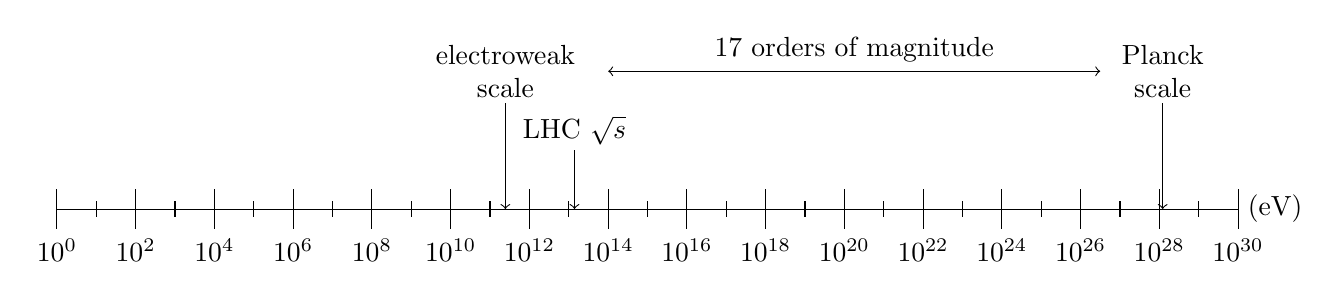
\begin{tikzpicture}
  % Axis
  \draw (0,0) -- (15,0) node[right] {(eV)};
  \draw (0,-0.25) -- (0,0.25);
  \node[below] at (0,-0.25) {$10^0$};

  \foreach \i in {1,...,15}
  {
    % Ticks
    \pgfmathsetmacro{\y}{\i-0.5}
    \draw (\i,-0.25) -- (\i,0.25);
    \draw (\y,-0.1) -- (\y,0.1);

    % Numerical labels
    \pgfmathtruncatemacro{\x}{\i*2}
    \node[below] at (\i,-0.25) {$10^{\x}$};
  }

  % Labels
  \draw[->] (5.695,1.75) node[fill=white,inner sep=2pt,align=center] {electroweak\\scale} -- (5.695,0);
  \draw[->] (6.573,1) node[fill=white,inner sep=2pt] {LHC $\sqrt{s}$} -- (6.573,0);
  \draw[->] (14.043,1.75) node[fill=white,inner sep=2pt,align=center] {Planck\\scale} -- (14.043,0);
  \draw[<->] (7,1.75) -- (13.25,1.75) node[pos=0.5,above] {17 orders of magnitude};
\end{tikzpicture}

  \caption{
    Comparison between the electroweak scale, LHC center of mass energy $\sqrt{s}$, and Planck scale in eV.
    The hierarchy problem arises due to the unexplained difference between the Planck scale at which gravitational effects become apparent and the energy scale at which electroweak symmetry breaking occurs, which are 17 orders of magnitude apart.
  }
  \label{fig:hierarchy}
\end{figure}

% Addressing the hierarchy problem
In the absence of some mechanism that resolves this problem, we are left with having to fine-tune parameters of the Standard Model in order to account for the large difference between the EW scale and the Planck scale. % Check wording
On the other hand, some BSM theories seek to address this problem in a more natural manner that does not require such fine-tuning.
Such theories result in new physics that may be experimentally verified, with some predicting the existence of new heavy particles that could be detected in collision events at the LHC.
% Possibly mention the hierarchy problem in terms of renormalizing the Higgs mass

% Possibly irrelevant and may need to comment out
\subsubsection{Supersymmetric Theories}

% Supersymmetry
Supersymmetry extends the notion of local symmetry to fermionic and bosonic fields, suggesting that there are symmetry transformations that mix the fields into each other~\cite{Wess197452}.
SUSY theories suggest that every known fermion has a corresponding bosonic partner, and every known boson has a corresponding fermionic partner.
For example, the electron would have a spin-0 supersymmetric partner known as the `selectron', and there would be other supersymmetric partners such as `squarks' and `sneutrinos'~\cite{Martin_1998}.
Bosonic particles would have partners such as the `photoino', `gluino', 'wino', and 'zino'.
However, one main issue is that no such supersymmetric partners have been identified, and the simplest models predict that they should have the same mass as their SM partners.
This suggests that if there is a supersymmetric theory that turns out to be correct, there must be a spontaneously broken symmetry mechanism that causes supersymmetric partners to differ in mass from their SM partners~\cite{dine_2007}.
% Elaborate on ongoing searches and particles that could be produced

\subsubsection{Grand Unified Theories}

% Grand unified theories
Grand Unified Theories are largely inspired by the success of the electroweak unification.
In the same way that the electromagnetic and weak forces become a single interaction at a particular energy scale, GUTs aim to unify the strong force with the other two forces of the Standard Model.
This requires a symmetry group that contains the $SU(3)_C\times SU(2)_L\times U(1)_Y$ group as a subgroup.
The first example of a GUT was the Georgi-Glashow model that was based on the $SU(5)$ group~\cite{PhysRevLett.32.438}.
A unique aspect of such theories is that they often predict that the proton is unstable and can decay due to new gauge bosons that couple quarks to leptons\footnotemark.
\footnotetext{Such particles are often called `leptoquarks'~\cite{Diaz_2017}.}
However, proton decay has not been observed~\cite{PhysRevLett.81.3319}, and the current lower bound for the lifetime of the proton is inconsistent with the Georgi-Glashow model.
Despite this, there are still other models based on more complex groups, such as $E_6$~\cite{Hewett1989193} or $SO(10)$~\cite{Cveti__1997}, that are candidates for further investigation.
% Elaborate on how such theories resolve the hierarchy problem

\subsubsection{Warped Extra Dimensions}

% Warped extra dimensions
There are many BSM theories that suggest that there are extra spatial dimensions, some of which are based on work done well before the formulation of the Standard Model.
Classical Kaluza-Klein theory has its roots in the early 20th century, and like RS models, its main feature is the addition of a fourth spatial dimension~\cite{1921spaw966K}.
It is a unified field theory that combines gravity and electromagnetism, and it rests on the idea that the extra spatial dimension is compactified in such a way that makes it experimentally difficult to observe.
The integration of electromagnetism into the theory neatly follows from symmetry considerations due to the extra spatial dimension.

% Randall-Sundrum models
Such work involving extra dimensions has paved the way for later theoretical developments in the field.
Randall-Sundrum (RS) models are examples of this, which propose that there is an extra fourth spatial dimension that has a strongly warped geometry~\cite{PhysRevLett.83.4690}.
These models are based on the idea that the spatial dimensions of the universe are restricted to a brane embedded within a higher-dimensional space known as the ``bulk.''
In such a framework, the elementary particles---except for the graviton---are localized in (3+1)-dimensional branes, while the graviton is able to propagate in the bulk.
The warped geometry is such that there are two branes in these models: the Tevbrane where the SM particles are localized, and the Planckbrane where the gravitational force becomes much stronger.
% Possibly elaborate

\section{Search for a Heavy Diboson Resonance}
\label{sec:VBF}

% Search for a heavy diboson resonance
This thesis presents results on the search for a new heavy $X$ resonance produced through vector boson fusion (VBF), with the resonance then decaying into a pair of bosons as part of efforts to explore BSM physics at the LHC.
The decays of interest are $X\to WV$ and $X\to WH$, where $V=W,Z$ is any of the two massive electroweak vector bosons and $H$ is a Higgs boson.
We consider semileptonic final event states in which the $W$ decays leptonically via $W\to \ell\nu$, the other vector boson decays hadronically through the process $V\to q\bar{q}^{(\prime)}$ and is reconstructed as a single massive jet, and there are two forward-facing jets resulting from the VBF production process.

% Previous work
This work is motivated in part by models such as those mentioned in subsection~\ref{subsec:BSM}, and is a continuation of a previous search using the 2016 data collected by the LHC during Run 2~\cite{Sirunyan_18}.
The previous analysis was conducted using only two benchmark signal models, and it was agnostic to the method of production for an $X$ resonance.
This work instead uses four benchmark signal models and is specific to a VBF production mode for the heavy resonance.

\subsection{Benchmark Models}

% List of signal models used
The search conducted in this work is model independent---it is not specific to a signal model and can cover many possibilities for an $X$ resonance.
However, benchmark models based on the BSM theories described in subsection~\ref{subsec:BSM} are used in order to model hypothetical collision events in the LHC that result in the final event states of interest.
The structure of these events then informs us about making our selection cuts for our search, as will be discussed in chapter~\ref{chap:analysis}.
This search covers spin-0, spin-1, and spin-2 bosonic resonances, and is based off of the following benchmark models:
\begin{enumerate}
  \item \textbf{Spin-0 Kaluza-Klein Radion:} A neutral scalar boson appearing in RS models that can decay to the vector bosons $W$ and $Z$ via $\mathrm{Rad}\to WW$ and $\mathrm{Rad}\to ZZ$~\cite{Goldberger_1999,Goldberger_2000}.
  \item \textbf{Spin-1 $W'$/$Z'$ Boson:} A heavier version of the spin-1 $W$ and $Z$ bosons that can decay via $W'\to WZ$, $W'\to WH$, and $Z'\to WW$~\cite{Pappadopulo_2014}.
  \item \textbf{Spin-2 Bulk Graviton:} A spin-2 resonance from a bulk RS model that decays via $G_\mathrm{bulk}\to WW$ or $G_\mathrm{bulk}\to ZZ$~\cite{Fitzpatrick_2007,PhysRevD.76.036006}.
\end{enumerate}

% Motivation for using signal models
These benchmarks cover a wide range of possibilities for candidate BSM bosonic resonances to be discovered.
Despite the variety in signal models, they may all result in similar semileptonic final states, thereby allowing the analysis to be model independent.
Furthermore, based on previous searches that have been conducted, they are all expected to be in the TeV mass range. % Citations (check 2018 paper that references this in the introduction)

\subsection{Expected Event Structure}
\label{subsec:expEvent}

% Event structure
The decay processes $X\to WV\to\ell\nu q\bar{q}^{(\prime)}$ and $X\to WH\to\ell\nu b\bar{b}$ were selected due to the fact that one-lepton events are ideal for such an analysis, as the final states that are generated provide a clean signal that suppresses background.
The VBF production channel was also selected to further suppress background and identify signal events since the VBF process uniquely results in forward-facing jets~\cite{rauch2016vectorboson}.
Examples of Feynman diagrams for the VBF production process of an $X$ resonance with the resulting final states can be seen in figure~\ref{fig:vbfFeynman}.
Such a process has been used in the past as one of the discovery channels for the Higgs boson, and it remains an important class of events at the LHC.

\begin{figure}[htbp]
  \centering
  % !TEX root = ../../thesis.tex
\begin{tikzpicture}
  \begin{feynman}
    % Vertices
    \coordinate (q1) at (-1.5,1.25);
    \coordinate (q2) at (0,1);
    \coordinate (q3) at ($(q2)+(11.5:4.75)$);
    \coordinate (q4) at (-1.5,-1.25);
    \coordinate (q5) at (0,-1);
    \coordinate (q6) at ($(q5)+(-11.5:4.75)$);
    \coordinate (v1) at (1,0);
    \coordinate (x1) at (2.25,0);
    \coordinate (v2) at (3.5,0.75);
    \coordinate (v3) at (3.5,-0.75);
    \coordinate (q7) at ($(v2)+(15:1.25)$);
    \coordinate (q8) at ($(v2)+(-15:1.25)$);
    \coordinate (l1) at ($(v3)+(15:1.25)$);
    \coordinate (l2) at ($(v3)+(-15:1.25)$);

    \coordinate (q9) at ($(q1)+(8.5,0)$);
    \coordinate (q10) at ($(q2)+(8.5,0)$);
    \coordinate (q11) at ($(q3)+(8.5,0)$);
    \coordinate (q12) at ($(q4)+(8.5,0)$);
    \coordinate (q13) at ($(q5)+(8.5,0)$);
    \coordinate (q14) at ($(q6)+(8.5,0)$);
    \coordinate (v4) at ($(v1)+(8.5,0)$);
    \coordinate (x2) at ($(x1)+(8.5,0)$);
    \coordinate (v5) at ($(v2)+(8.5,0)$);
    \coordinate (v6) at ($(v3)+(8.5,0)$);
    \coordinate (q15) at ($(q7)+(8.5,0)$);
    \coordinate (q16) at ($(q8)+(8.5,0)$);
    \coordinate (l3) at ($(l1)+(8.5,0)$);
    \coordinate (l4) at ($(l2)+(8.5,0)$);

    % Lines
    \draw[fermion] (q1) -- (q2);
    \draw[fermion] (q2) -- (q3);
    \draw[fermion] (q4) -- (q5);
    \draw[fermion] (q5) -- (q6);
    \draw[boson] (q2) -- (v1) node[pos=0.65,xshift=-0.5cm] {$Z$};
    \draw[boson] (q5) -- (v1) node[pos=0.65,xshift=-0.5cm] {$Z$};
    \draw[boson] ($(v1)+(0,-0.025)$) -- ($(x1)+(0,-0.025)$);
    \draw[boson] ($(v1)+(0,0.025)$) -- ($(x1)+(0,0.025)$) node[pos=0.5,above] {$X$};
    \draw[boson] (x1) -- (v2) node[pos=0.9,xshift=-0.5cm] {$W$};
    \draw[boson] (x1) -- (v3) node[pos=0.9,xshift=-0.5cm] {$W$};
    \draw[fermion] (v2) -- (q7);
    \draw[fermion] (q8) -- (v2);
    \draw[fermion] (v3) -- (l1);
    \draw[fermion] (l2) -- (v3);

    \draw[fermion] (q9) -- (q10);
    \draw[fermion] (q10) -- (q11);
    \draw[fermion] (q12) -- (q13);
    \draw[fermion] (q13) -- (q14);
    \draw[boson] (q10) -- (v4) node[pos=0.65,xshift=-0.5cm] {$W$};
    \draw[boson] (q13) -- (v4) node[pos=0.65,xshift=-0.5cm] {$Z$};
    \draw[boson] (v4) -- (x2) node[pos=0.5,above] {$X$};
    \draw[scalar] (x2) -- (v5) node[pos=0.9,xshift=-0.5cm] {$H$};
    \draw[boson] (x2) -- (v6) node[pos=0.9,xshift=-0.5cm] {$W$};
    \draw[fermion] (v5) -- (q15);
    \draw[fermion] (q16) -- (v5);
    \draw[fermion] (v6) -- (l3);
    \draw[fermion] (l4) -- (v6);

    % Blobs
    \fill[white] (v1) circle (0.2);
    \fill[white] (x1) circle (0.2);
    \draw[pattern=north west lines] (v1) circle (0.2);
    \draw[pattern=north west lines] (x1) circle (0.2);

    \fill[white] (v4) circle (0.2);
    \fill[white] (x2) circle (0.2);
    \draw[pattern=north west lines] (v4) circle (0.2);
    \draw[pattern=north west lines] (x2) circle (0.2);

    % Labels
    \node[anchor=mid,left] at (q1) {$q''$};
    \node[anchor=mid,left] at (q4) {$q'''$};
    \node[anchor=mid,right] at (q3) {$q''$};
    \node[anchor=mid,right] at (q6) {$q'''$};
    \node[anchor=mid,right] at (q7) {$q$};
    \node[anchor=mid,right] at (q8) {$\bar{q}'$};
    \node[anchor=mid,right] at (l1) {$\ell$};
    \node[anchor=mid,right] at (l2) {$\nu$};

    \node[anchor=mid,left] at (q9) {$q'$};
    \node[anchor=mid,left] at (q12) {$q'''$};
    \node[anchor=mid,right] at (q11) {$q''$};
    \node[anchor=mid,right] at (q14) {$q'''$};
    \node[anchor=mid,right] at (q15) {$b$};
    \node[anchor=mid,right] at (q16) {$\bar{b}$};
    \node[anchor=mid,right] at (l3) {$\ell$};
    \node[anchor=mid,right] at (l4) {$\nu$};
  \end{feynman}
\end{tikzpicture}

  \caption{
    Feynman diagrams for production via vector boson fusion of a neutral spin-2 resonance $X$ decaying to the final state $\ell\nu q\bar{q}'$ (left), and a charged spin-1 resonance decaying to the final state $\ell\nu b\bar{b}$ (right), both with additional forward-facing jets due to the VBF production process.
    The search for an $X$ boson will involve looking for a final state in which there are jets from the VBF production process present, along with a single merged jet from the $V$/$H$ boson, and a lepton $\ell$ with its corresponding neutrino $\nu$ produced from the $W$ decay.
  }
  \label{fig:vbfFeynman}
\end{figure}

% Event topology
Because the expected mass of the bosonic resonance lies in the TeV range, the final event state has a highly boosted topology, which is illustrated in figure~\ref{fig:eventTop}.
The two initial state quarks from the VBF process in the diagram of figure~\ref{fig:vbfFeynman} result in two forward-facing jets in the final state that are highly energetic and collimated.
Meanwhile, the lepton-neutrino pair from the $W\to\ell\nu$ decay will have momenta opposite to that of the jet that results from the hadronic decay of the $V$/$H$ boson.
The jet from the $V\to q\bar{q}^{(\prime)}$ or $H\to b\bar{b}$ decay will also have two-pronged substructure since the decay results in a quark-antiquark pair.
Lastly, both the lepton-neutrino pair and the jet will be highly collimated since the $W$ and $V$/$H$ bosons that produced them will have momenta of several hundred GeV or above.

\begin{figure}[htbp]
  \centering
  % !TEX root = ../../thesis.tex

\begin{tikzpicture}
  % Axis
  \draw[->] (-6,0) -- (6,0) node[right] {$z$};

  % Leptons
  \draw[->,thick] (0,0) -- (105:3) node[left] {$\ell$};
  \draw[->,thick] (0,0) -- (75:3) node[right] {$\nu$};

  % Main jet
  \draw[rotate around={180:(0,0)},dotted,thick] (0,2) ellipse (1.3 and 0.4);
  \draw[rotate around={180:(0,0)},dotted,thick] (0,0) -- (56.427:2.3);
  \draw[rotate around={180:(0,0)},dotted,thick] (0,0) -- (123.573:2.3);

  % Sub jets
  \draw[rotate around={180:(0,0)},dotted,thick] (0.5,2) ellipse (0.4 and 0.1);
  \draw[rotate around={180:(0,0)},dotted,thick] (0,0) -- (65.715:2.18);
  \draw[rotate around={180:(0,0)},dotted,thick] (0,0) -- (87.135:2);
  \draw[rotate around={180:(0,0)},dotted,thick] (-0.5,2) ellipse (0.4 and 0.1);
  \draw[rotate around={180:(0,0)},dotted,thick] (0,0) -- (92.865:2);
  \draw[rotate around={180:(0,0)},dotted,thick] (0,0) -- (114.285:2.18);

  % VBF Jets
  \draw[rotate around={80:(0,0)},dotted,thick] (0,4) ellipse (0.5 and 0.1);
  \draw[rotate around={80:(0,0)},dotted,thick] (0,0) -- (82.875:4.03);
  \draw[rotate around={80:(0,0)},dotted,thick] (0,0) -- (97.125:4.03);
  \draw[rotate around={260:(0,0)},dotted,thick] (0,4) ellipse (0.5 and 0.1);
  \draw[rotate around={260:(0,0)},dotted,thick] (0,0) -- (82.875:4.03);
  \draw[rotate around={260:(0,0)},dotted,thick] (0,0) -- (97.125:4.03);

  % Labels
  \node[anchor=mid] at (257.5:2.75) {$q$};
  \node[anchor=mid] at (282.5:2.75) {$\bar{q}^{(\prime)}$};
  \node[anchor=mid] at (170:4.5) {$q^{(\prime)}$};
  \node[anchor=mid] at (350:4.5) {$q^{(\prime)}$};

\end{tikzpicture}

  \caption{
    Illustration of event topology for VBF collision events of interest in the CMS detector.
    The semi-leptonic final state produces a $W$ boson that decays via $W\to\ell\nu$ and produces the lepton-neutrino pair.
    Opposite to that is a single massive jet with two-pronged substructure that is produced via $V\to q\bar{q}^{(\prime)}$ or $H\to b\bar{b}$.
    Finally, the VBF production process results in two forward-facing jets, labeled by $q^{(\prime)\prime\prime}$ and $q^{(\prime)\prime\prime\prime}$.
  }
  \label{fig:eventTop}
\end{figure}
